%%%%%%%%%%%%%%%%%%%%%%%%%%%%%%%%%%%%%%%%%
% Short Sectioned Assignment LaTeX Template Version 1.0 (5/5/12)
% This template has been downloaded from: http://www.LaTeXTemplates.com
% Original author:  Frits Wenneker (http://www.howtotex.com)
% License: CC BY-NC-SA 3.0 (http://creativecommons.org/licenses/by-nc-sa/3.0/)
%%%%%%%%%%%%%%%%%%%%%%%%%%%%%%%%%%%%%%%%%

%----------------------------------------------------------------------------------------
%	PACKAGES AND OTHER DOCUMENT CONFIGURATIONS
%----------------------------------------------------------------------------------------

\documentclass[paper=a4, fontsize=11pt]{scrartcl} % A4 paper and 11pt font size

% ---- Entrada y salida de texto -----

\usepackage[T1]{fontenc} % Use 8-bit encoding that has 256 glyphs
\usepackage[utf8]{inputenc}
%\usepackage{fourier} % Use the Adobe Utopia font for the document - comment this line to return to the LaTeX default


\usepackage[utf8]{inputenc}
\usepackage[T1]{fontenc}
\usepackage[spanish]{babel}
\usepackage{times}

\usepackage{color}
\definecolor{gray97}{gray}{.97}
\definecolor{gray75}{gray}{.75}
\definecolor{gray45}{gray}{.45}

\usepackage{listings}
\lstset{ frame=Ltb,
	framerule=0pt,
	aboveskip=0.5cm,
	framextopmargin=3pt,
	framexbottommargin=3pt,
	framexleftmargin=0.4cm,
	framesep=0pt,
	rulesep=.4pt,
	backgroundcolor=\color{gray97},
	rulesepcolor=\color{black},
	%
	stringstyle=\ttfamily,
	showstringspaces = false,
	basicstyle=\small\ttfamily,
	commentstyle=\color{gray45},
	keywordstyle=\bfseries,
	%
	numbers=left,
	numbersep=15pt,
	numberstyle=\tiny,
	numberfirstline = false,
	breaklines=true,
}

% minimizar fragmentado de listados
\lstnewenvironment{listing}[1][]
{\lstset{#1}\pagebreak[0]}{\pagebreak[0]}

\lstdefinestyle{consola}
{basicstyle=\scriptsize\bf\ttfamily,
	backgroundcolor=\color{gray75},
}

\lstdefinestyle{C}
{language=C,
}
% ---- Idioma --------

\usepackage[spanish, es-tabla]{babel} % Selecciona el español para palabras introducidas automáticamente, p.ej. "septiembre" en la fecha y especifica que se use la palabra Tabla en vez de Cuadro
% ---- Otros paquetes ----

\usepackage{amsmath,amsfonts,amsthm} % Math packages
%\usepackage{graphics,graphicx, floatrow} %para incluir imágenes y notas en las imágenes
\usepackage{graphics,graphicx, float} %para incluir imágenes y colocarlas

% Para hacer tablas comlejas
%\usepackage{multirow}
%\usepackage{threeparttable}

%\usepackage{sectsty} % Allows customizing section commands
%\allsectionsfont{\centering \normalfont\scshape} % Make all sections centered, the default font and small caps

\usepackage{fancyhdr} % Custom headers and footers
\pagestyle{fancyplain} % Makes all pages in the document conform to the custom headers and footers
\fancyhead{} % No page header - if you want one, create it in the same way as the footers below
\fancyfoot[L]{} % Empty left footer
\fancyfoot[C]{} % Empty center footer
\fancyfoot[R]{\thepage} % Page numbering for right footer
\renewcommand{\headrulewidth}{0pt} % Remove header underlines
\renewcommand{\footrulewidth}{0pt} % Remove footer underlines
\setlength{\headheight}{13.6pt} % Customize the height of the header

\numberwithin{equation}{section} % Number equations within sections (i.e. 1.1, 1.2, 2.1, 2.2 instead of 1, 2, 3, 4)
\numberwithin{figure}{section} % Number figures within sections (i.e. 1.1, 1.2, 2.1, 2.2 instead of 1, 2, 3, 4)
\numberwithin{table}{section} % Number tables within sections (i.e. 1.1, 1.2, 2.1, 2.2 instead of 1, 2, 3, 4)

\setlength\parindent{0pt} % Removes all indentation from paragraphs - comment this line for an assignment with lots of text

\newcommand{\horrule}[1]{\rule{\linewidth}{#1}} % Create horizontal rule command with 1 argument of height


\begin{document}
\title{
\normalfont \normalsize 
\textsc{{\bf Aprendizaje Automático (2015-16) \\ Grado en Ingeniería Informática \\ Universidad de Granada} \\ [25pt] % Your university, school and/or department name(s)
\horrule{0.5pt} \\[0.4cm] % Thin top horizontal rule
\huge Informe Trabajo de Prácticas 1 \\ % The assignment title
\horrule{2pt} \\[0.5cm] % Thick bottom horizontal rule
}}
\author{Miguel López Campos} % Nombre y apellidos

\date{\normalsize\today} % Incluye la fecha actual
%----------------------------------------------------------------------------------------
% DOCUMENTO
%----------------------------------------------------------------------------------------


	
	\maketitle % Muestra el Título
	\newpage %inserta un salto de página
	
	\tableofcontents % para generar el índice de contenidos
	\listoffigures

	
	\newpage
	
	\
	
	\section{Ejercicio 5.2: Generación y Visualización de datos}
	\subsection{Apartados 1, 2, 3 y 4}
	Para crear las funciones simula\_unif y simula\_gauss he usado sapply. En sapply introduzco como argumentos un array que indica el número de veces que quiero que se ejecute la función deseada (runif o rnorm en nuestro caso), así como los argumentos de la función deseada. sapply además intenta simplificar lo máximo posible la estructura de datos en la que se devuelve el resultado. 
	\\
	
	Tras las ejecuciones de simula\_unif y simula\_gauss obtenemos las siguientes gráficas.
	\begin{figure} [H]
	\centering
	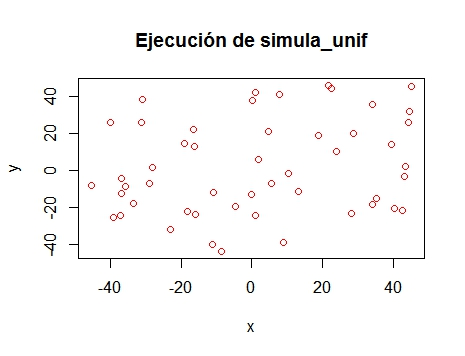
\includegraphics[width=0.7\linewidth]{simulaunif}
	\caption{Ejecución de simula unif}
	\label{fig:simula_unif}
	\end{figure}

	\begin{figure} [H]
	\centering
	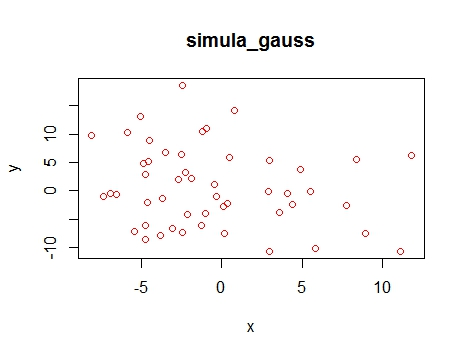
\includegraphics[width=0.7\linewidth]{simulagauss}
	\caption{Ejecución de simula Gauss}
	\label{fig:simulagauss}
	\end{figure}
	
	
	\subsection{Apartado 5: Construir recta aleatoria}
	Para crear la recta hay que generar dos puntos de forma aleatoria. La recta resultante será la que pasa por estos dos puntos. Teniendo en cuenta que la ecuación de una recta es y = ax+b, podemos resolver un sistema de ecuaciones cuyas incógnitas sean 'a' y 'b'. En la función simula\_recta resuelvo este sistema de ecuaciones y devuelvo una lista con los valores aleatorios de 'a' y 'b'.
	\\
	
	\begin{lstlisting}
	simula_recta <- function()
	{
		intervalo <- c(-50,50)
		p <- simula_unif(N=2, dim=2, c(-50,50))
		a <- (p[2,2]-p[2,1])/(p[1,2]-p[1,1])
		b <- p[2,1]-p[1,1]*a
		return(list(a,b))
	}
	\end{lstlisting}
	
	\subsection{Apartado 6: Etiquetado de muestra aleatoria}
	Para realizar este apartado primero uso la función simula\_unif para generar 1000 puntos de 2D. Al devolverme una matriz, convierto ésta a un data frame para tener una representación de la estructura de datos más clara, poniéndole de nombre a las columnas 'x' e 'y'. Simulo la recta y etiqueto siguiendo la función f(x, y) = y - ax - b. En la gráfica se puede ver el resultado. Los puntos verdes son +1 y los rojos -1.
	\begin{figure}[H]
	\centering
	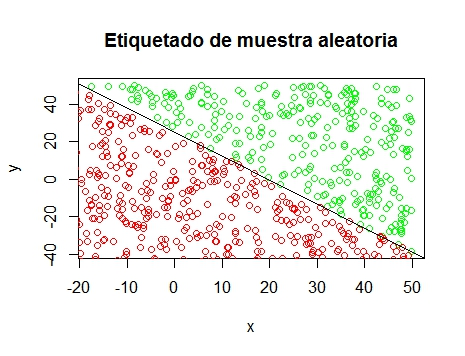
\includegraphics[width=0.7\linewidth]{apartado6}
	\caption{Etiquetado de muestra aleatoria con recta aleatoria}
	\label{fig:apartado6}
	\end{figure}
	
	\subsection{Apartado 7: Etiquetado para funciones no lineales}
	Las funciones son las siguientes (verde +1, rojo -1)
	\begin{itemize}
	\item f(x, y) = (x - 10)^2 + (y - 20)^2 - 400
	\end{itemize}
	
	\begin{figure} [H]
	\centering
	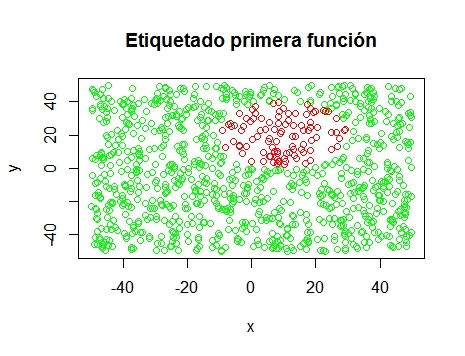
\includegraphics[width=0.7\linewidth]{primerafuncion}
	\caption{Apartado 7: primera funcion}
	\label{fig:primerafuncion}
	\end{figure}
	
	\begin{itemize}
		\item f(x, y) = 0.5(x + 10)^2 + (y - 20)^2 - 400
	\end{itemize}
	
	\begin{figure} [H]
	\centering
	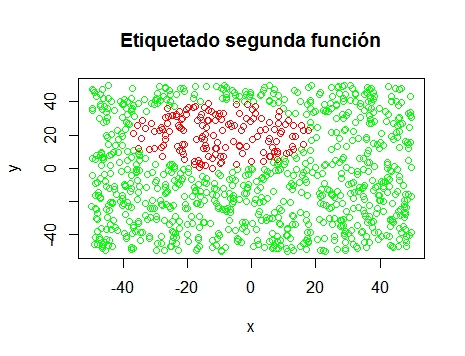
\includegraphics[width=0.7\linewidth]{etiquetasegundafuncion}
	\caption{Apartado 7: segunda funcion}
	\label{fig:etiquetasegundafuncion}
	\end{figure}

	\begin{itemize}
		\item f(x, y) = 0.5(x - 10)^2 - (y + 20)^2 - 400
	\end{itemize}
	
	\begin{figure} [H]
	\centering
	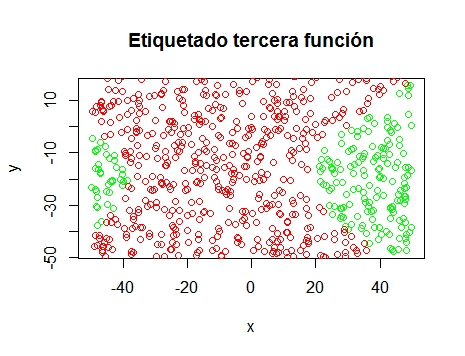
\includegraphics[width=0.7\linewidth]{tercerafuncion}
	\caption{Apartado 7: tercera funcion}
	\label{fig:tercerafuncion}
	\end{figure}

	\newpage
	
	\begin{itemize}
		\item f(x, y) = y - 20x^2 - 5x + 3
	\end{itemize}
	
	\begin{figure} [H]
		\centering
		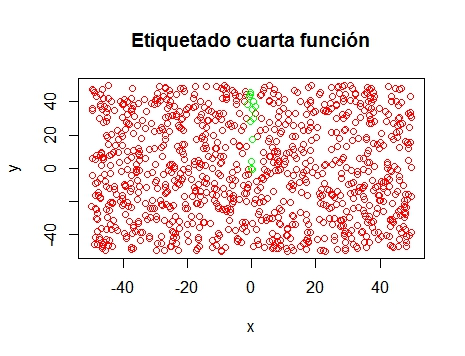
\includegraphics[width=0.7\linewidth]{cuartafuncion}
		\caption{Apartado 7: cuarta funcion}
		\label{fig:cuarta funcion}
	\end{figure}
	
	Sobre estas funciones se puede deducir que no son lineales, es decir, no se pueden dividir los puntos etiquetados mediante una recta.
	
	\subsection{Apartado 8: Ruido en la muestra}
	Para cambiar el 10\% de los puntos positivos por negativos y viceversa he creado la siguiente función en la que lo que hago es extraer un 10\% de cada uno de los etiquetados mediante la función sample. Entonces lo que hago es tener un array de probabilidad que es probs y asigno probabilidad 0 a los negativos y 1 a los positivos (para cambiar negativos, a la inversa). De entrada a sample también le introduzco un vector (que son los índices del array de etiquetas) y la longitud de la muestra aleatoria de índices que quiero sacar (en mi caso el 10\%). Para esos índices obtenidos de manera aleatoria, cambio su etiqueta:
	
	\newpage
	
	\begin{lstlisting}
	change_muestra <- function(x)
	{
	
		n_positivos <- as.integer(length(x[x>0])/10)
		probs <- rep(1, length(x))
		probs[x<0] <- 0
		#Con sample obtengo aleatoriamente un vector de índices aleatorios correspondientes
		#con el 10% de las etiquetas positivas. Estos índices los usaré para cambiar la etiqueta
		ind_aleatorios <- sample(x=(1:length(x)), prob=probs, size=n_positivos)
		new_muestra <-x
		new_muestra[ind_aleatorios] <- -1
		
		n_negativos <- as.integer(length(x[x<0])/10)
		probs <- rep(1, length(x))
		probs[x>0] <- 0
		ind_aleatorios <- sample(x=(1:length(x)), prob=probs, size=n_negativos)
		new_muestra[ind_aleatorios] <- 1
		
		return(new_muestra)
	}

	\end{lstlisting}
	
	\begin{figure} [H]
	\centering
	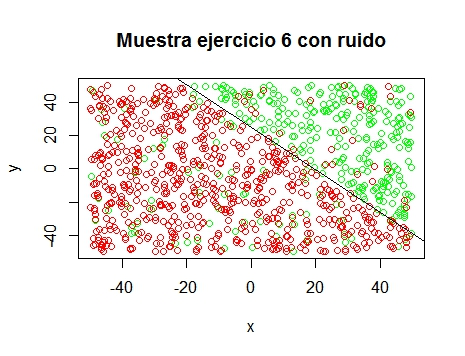
\includegraphics[width=0.7\linewidth]{ejercicio8}
	\caption{Hemos aplicado ruido}
	\label{fig:ejercicio8}
	\end{figure}

	\newpage
	
	Como consecuencia de esta modificación, estamos introduciendo ruido a la muestra. Esto supone una pérdida de lineabilidad en los etiquetados y por consecuente una dificultad a la hora de realizar el aprendizaje.
	
	\section{Ejercicio 5.3: Ajuste del Algoritmo Perceptron}
	\subsection{Apartado 1: Implementación}
	En mi implementación introduzco el vector de pesos inicial de manera separada donde el término de w independiente lo introduzco también independientemente. Esto lo hago para no tener que añadir siempre una columna de 1's a la matriz que introduzco de entrada. Dentro de la función ajusta\_PLA tenemos un bucle while externo. Éste se ejecutará mientras haya cambios en el vector de pesos y mientras que no se supere el umbral dado como argumento. Dentro de este while tenemos un for que recorrerá todos los elementos de la muestra y comprobará si con ese vector de pesos está bien ajustado. Si no lo está, cambia el vector de pesos. Una vez acaba la función devolvemos el número de iteraciones necesarias para que converga a una solución y el vector de pesos.
	
	\begin{lstlisting}
	ajusta_PLA <- function(datos, label, max_iter, vini, b)
	{
		change <- 1
		w <- vini
		iter <- 0
		while(change == 1 && iter < max_iter)
		{  
		
			change <- 0
			
			for(i in seq_along(label))
			{
				if(sign(sum(datos[i,]*w)+b)!=sign(label[i]))
				{
				change <- 1
				w <- w + datos[i,]*label[i]
				b <- b + label[i]
				}
			}
			
			iter <- iter+1
		}
		
		length(w) <- length(w)+1
		w[length(w)] <- b
		cat("Se han necesitado ")
		cat(iter)
		cat(" iteraciones")
		
		return(list(iter,w))
	}
\end{lstlisting}


\subsection{Apartado 2: Ejecución PLA}
Para hacer el número de iteraciones medio para que converja, hago un bucle for que se repita 10 veces y en él genero de forma aleatoria el vector de pesos inicial. En la figura hay un ejemplo de un número medio de iteraciones. Esto es un claro indicativo de que el vector inicial de pesos es importante a la hora de eficiencia y, cuando los datos no sean linealmente separables, lo será también para el resultado. Adjunto también una gráfica del resultado de una de las estimaciones.
\begin{figure} [H]
\centering
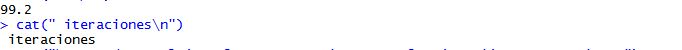
\includegraphics[width=0.7\linewidth]{iters}
\caption{Número medio de iteraciones}
\label{fig:iters}
\end{figure}

\begin{figure} [H]
\centering
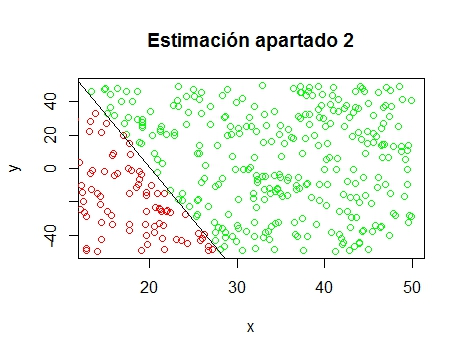
\includegraphics[width=0.7\linewidth]{ei}
\caption{Estimación ejecutando PLA. Como vemos es muy buena.}
\label{fig:ei}
\end{figure}


\subsection{Apartado 3: Ejecución PLA datos con ruido}
Para realizar este apartado lo que hago es inicializar en cada una de las pruebas el vector de pesos inicial a 0. He obtenido, para un número máximo de iteraciones N=10, 187 errores; para N=100, 197 errores, y para N=1000, 215 errores. Esto nos indica que el perceptrón, cuando no hay una clara separabilidad lineal entre los datos (en este caso debido al ruido), aunque haga más iteraciones no tiene por qué dar una solución mejor.

\subsection{Apartado 4: Ejecución PLA datos no linealmente separables}
En este ejercicio realizo el mismo procedimiento que en el apartado anterior pero con la muestra del apartado 7 (primera función) del anterior ejercicio. En este caso obtengo para N=10, 418 errores. Para N=100, 112 errores, y para N=1000 340 errores. Como vemos, tenemos un porcentaje de error muy alto, incluso más que en el apartado anterior. Como hemos visto antes, la función del ejercicio 7 era no linealmente separable para las muestras. Por esto tenemos un porcentaje de error tan alto dentro de la muestra.

\subsection{Apartado 5: Modificación de PLA}
Para este apartado he realizado la siguiente versión modificada de PLA:
\newpage

	\begin{lstlisting}
	ajusta_PLA_modificado <- function(datos, label, max_iter, vini, b)
	{
		change <- 1
		w <- vini
		iter <- 0
		while(change == 1 && iter < max_iter)
		{  
		
			change <- 0
			
			for(i in seq_along(label))
			{
			
			
				if(sign(sum(datos[i,]*w)+b)!=sign(label[i]))
				{
				change <- 1
				w <- w + datos[i,]*label[i]
				b <- b + label[i]
				}
			}
			positivos <- label>0
			plot(datos[positivos,], col="red")
			points(datos[!positivos,], col="green")
			abline(a=(-b/w[2]), b=(-w[1]/w[2]))
			Sys.sleep(0.1)
			
			iter <- iter+1
		}
		
		length(w) <- length(w)+1
		w[length(w)] <- b
		cat("Se han necesitado ")
		cat(iter)
		cat(" iteraciones")
		
		return(w)
	}
	\end{lstlisting}
	
	Lo que hago, es después de haber recorrido toda la muestra en una iteración, muestro una gráfica representando los puntos (verdes +1 y rojos -1) así como la recta obtenida a partir de los pesos que se han calculado en esa iteración. También pongo un sys.sleep para que nos de tiempo a visualizar la gráfica.
	\\
	\\
	
	En las dos siguientes figuras se ve la gráfica después de la primera iteración y la gráfica después de la segunda.
	\begin{figure}[H]
	\centering
	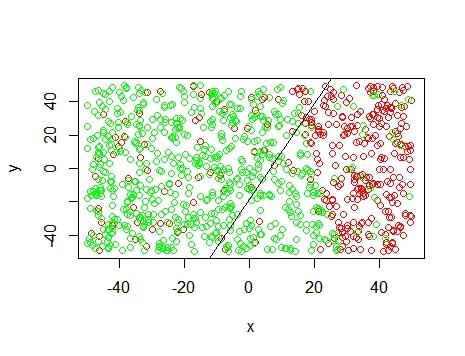
\includegraphics[width=0.7\linewidth]{iter1}
	\caption{Iteración 1}
	\label{fig:iter1}
	\end{figure}
	\begin{figure} [H]
	\centering
	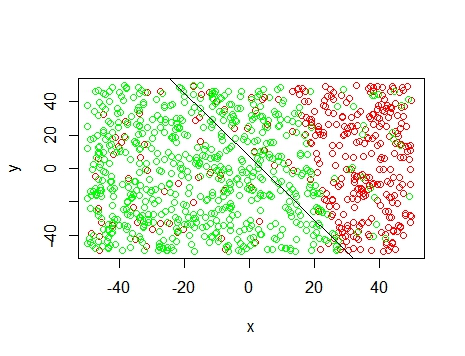
\includegraphics[width=0.7\linewidth]{iter2}
	\caption{Iteración 2}
	\label{fig:iter2}
	\end{figure}
	
	\subsection{Apartado 6: Mejora para funciones no lineales}
	Para mejorar el PLA para funciones no lineales, he implementado el pocket PLA, que es el siguiente:
	\begin{lstlisting}
	ajusta_PLA_MOD <- function(datos, label, t, max_iter_PLA)
	{
		vini <- c(0,0)
		b <- 0
		w <- c(vini,b)
		error_mejor <- 1
		
		for(i in 1:t)
		{
			data_tmp <- as.matrix(datos)
			w_temp <- ajusta_PLA(data_tmp,label, max_iter_PLA, w[1:2], w[3])[[2]]
			etiq_nuev <- datos$x*w_temp[1] + datos$y*w_temp[2] + w_temp[3]
			etiq_nuev[etiq_nuev>0] <- 1
			etiq_nuev[etiq_nuev<0] <- -1
			errores <- label!=etiq_nuev
			errores <- label[errores]
			error_nuevo <- length(errores)/length(label)
			
			if(error_nuevo < error_mejor)
			{
				error_mejor <- error_nuevo
				w <- w_temp
			}
		}
	
	return(w)
	}
	\end{lstlisting}
	La función lo que hace es, inicializando el vector de pesos a 0, calcular reiteradamente pesos con PLA. Si los pesos que calcula son mejores que los anteriormente calculados, entonces actualizamos y en la siguiente iteración el vector inicial de pesos para PLA serán los mejores pesos. Para la primera función del ejercicio 7 obtenemos el siguiente resultado.
	\begin{figure}
	\centering
	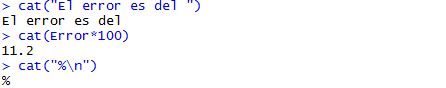
\includegraphics[width=0.7\linewidth]{error6}
	\caption{Error usando Pocket PLA sobre primera función del ejercicio 7}
	\label{fig:error6}
	\end{figure}
	Como vemos, el error es del 11\%, que comparado con el obtenido con PLA (41.8\%) es muchísimo mejor.

	\section{Ejercicio 5.4: Regresión lineal}
	\subsection{Apartados 1 y 2: Leer datos y visualizarlos}
	Para leer el fichero de datos usamos la función read.table. Asigno a una variable este conjunto de datos. Después creo las matrices de 16x16 y las pongo todas en una lista. Las etiquetas las meto en una lista a parte.
	\\
	Para visualizar la imagen, usamos la función image, introduciéndole como argumento la matriz deseada. En la figura se puede observar uno de los datos pintados.
	\begin{figure} [H]
	\centering
	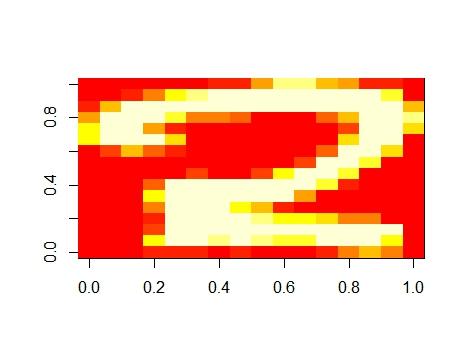
\includegraphics[width=0.7\linewidth]{datoimagen}
	\caption{Visualizamos uno de los datos del conjunto de datos}
	\label{fig:datoimagen}
	\end{figure}
	
	Como vemos los datos son dígitos pintados a mano. Para quedarnos solo con los 1's y los 5's, lo que hago es que desde la lista de etiquetas me quedo sólo con éstos con el siguiente trozo de código:
	\begin{lstlisting}
		accept1 <- labels_digits == 5
		accept2 <- labels_digits == 1
		accept <- accept1+accept2
		m <- m[as.logical(accept)]
		labels_digits <- labels_digits[as.logical(accept)]
	\end{lstlisting}


	\subsection{Apartados 3 y 4: Simetría e intensidad de los datos y representación}
	Para calcular la intensidad media de los datos uso sapply de la siguiente manera:
	\begin{lstlisting}
	data_means <- sapply(m,mean)
	\end{lstlisting}
	Ésto lo que hace es devolver la media de cada una de las matrices (los datos) que están en la lista 'm'.
	\\
	\\
	Para calcular la simetría empleo la siguiente función
	\begin{lstlisting}
	simmetry_function <- function(m)
	{
		sum <- 0
		for(i in 1:nrow(m))
		{
			for(j in 1:ncol(m))
			{
				sum <- sum + abs(m[i,j]-m[i,ncol(m)-j+1])
			}
		}
		
		sum <- -sum
		return(sum)
	}
	\end{lstlisting}
	En la función lo que hago es recorrer todas las filas de la matriz y para cada una de las columnas hago la sumatoria del valor absoluto de la diferencia de cada uno de los pixeles con el pixel que correspondería al mismo con la imagen invertida. Para aplicarla sobre todas las imágenes (cada uno de los datos de la muestra) empleo sapply.
	\\
	\\
	\newpage
	En la siguiente gráfica muestro los 5's de color verde y los 1's de color rojo.
	\begin{figure} [H]
	\centering
	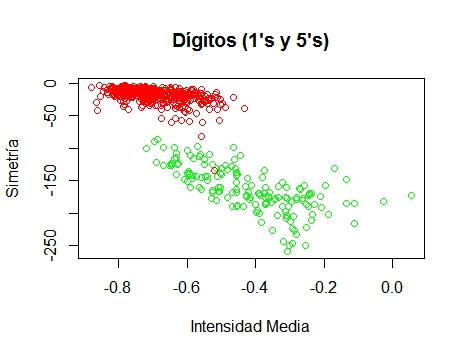
\includegraphics[width=0.7\linewidth]{digitos}
	\caption{Gráfica de los 1's y los 5's según simetría e intensidad media}
	\label{fig:digitos}
	\end{figure}

	\subsection{Apartados 5 y 6: Ajuste de regresión lineal}
	Para ajustar la regresión lineal he diseñado la siguiente función:
	\begin{lstlisting}
	Regress_lin <- function(datos, label)
	{
		descomposicion <- svd(datos)
		#La función diag construye una matriz diagonal a partir de un array
		D <- descomposicion$d
		for(i in 1:length(D))
		{
			if(D[i] > 10^-4)
			{
			D[i] <- 1/D[i]
			}else{D[i] <- 0}
		}
		D <- diag(D)
		V <- descomposicion$v
		U <- descomposicion$u
		#
		D <- t(D)
		pseudo_inverse <- V %*% D %*% t(U)
		w <- as.vector(pseudo_inverse %*% label)
	}
	\end{lstlisting}
	Primero hago la descomposición en valores singulares con svd. Para hacer la pseudoinversa de la matriz D, tengo que hacer el inverso de cada uno de sus elementos y después hacer la traspuesta. Pongo un umbral a partir del cual si es más pequeño, directamente pongo 0. Formo una matriz diagonal mediante la función diag. A continuación calculo la pseudo inversa de X y por último la multiplico por la matriz label que contendrá las etiquetas en una matriz de una sola columna. Devuelvo los pesos en un vector.
	
	\\
	
	\\
	
	En la siguiente figura muestro el resultado de aplicar regresión lineal sobre los datos de 1's y 5's con el código siguiente:
	\begin{lstlisting}
	datos <- data.frame(data_means, data_simmetry, rep(1,length(data_means)))
	datos <- as.matrix(datos)
	etiquetas <- matrix(labels_digits, ncol = 1)
	#Las etiquetas clasificaré los 5 como -1 y los 1's como +1
	cincos <- etiquetas==5
	etiquetas[cincos] = -1
	pesos <- Regress_lin(datos, etiquetas)
	\end{lstlisting}
	
	\begin{figure} [H]
	\centering
	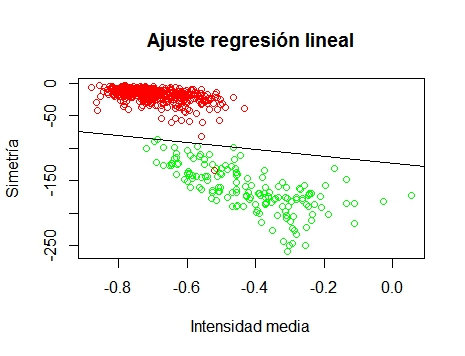
\includegraphics[width=0.7\linewidth]{regresionlineal}
	\caption{Regresión lineal sobre los datos de dígitos}
	\label{fig:regresionlineal}
	\end{figure}
	
	\subsection{Apartado 7}
	Para el apartado 'a' utilizo para etiquetar la función f(x,y) = y + ax +b , siendo 'a' y 'b' los coeficientes de una recta aleatoria. Aplico regresión lineal y calculo el error viendo el número de diferencias en relación al tamaño total de la muestra:
	\begin{lstlisting}
	  errores <- as.vector(label_7a)!=etiquetados
	  errores <- label_7a[errores]
	  Error[i] <- length(errores)/100
	\end{lstlisting}
	
	Obtengo un error muy bajo, del 1.514%:
	\begin{figure} [H]
	\centering
	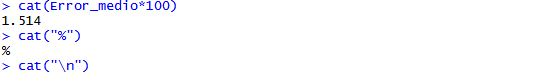
\includegraphics[width=0.7\linewidth]{errormedioa}
	\caption{Error medio apartado a}
	\label{fig:errormedioa}
	\end{figure}
	
	Para calcular el error fuera de la muestra, genero en cada iteración una muestra de 1000 elementos. La etiqueto con la función 'f' y después la etiqueto con los pesos obtenidos mediante la regresión lineal con la muestra de 100 elementos. Calculo el número de errores y lo pongo en relación a los 1000 elementos de la muestra. Al finalizar el experimento obtengo un error medio del 1.77\%. Como vemos tras varias ejecuciones, casi siempre el error fuera de la muestra es mayor que el de dentro, algo que es lógico. Además, al ser los datos linealmente separables, obtenemos un error muy bajo, por lo que el resultado de aplicar regresión lineal en estos casos es bueno.
	
	\begin{figure} [H]
	\centering
	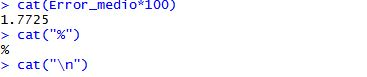
\includegraphics[width=0.7\linewidth]{errormediob}
	\caption{Error medio apartado b}
	\label{fig:errormediob}
	\end{figure}
	
	En el apartado c genero una muestra de tamaño N=10 y ajusto por regresión lineal. Los pesos obtenidos serán el vector de pesos inicial para el perceptrón. Como vemos se necesita de media muy pocas iteraciones para que converga (ver en la figura siguiente). Esto es debido a que al aplicar la regresión lineal estamos optimizando el error de dentro de la muestra, por lo que para el perceptrón será más fácil encontrar la solución.
	\begin{figure} [H]
	\centering
	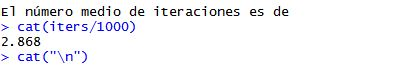
\includegraphics[width=0.7\linewidth]{iters7}
	\caption{Iteraciones medias perceptrón habiendo ajustado con regresión lineal antes}
	\label{fig:iters7}
	\end{figure}

	\subsection{Apartado 8: Transformaciones no lineales}
	Primero generamos la muestra de N=1000 de forma aleatoria y aplicamos ruido (usando sample como en un apartado anterior). He empleado el siguiente código para realizar el experimento:
	\begin{lstlisting}
	Error <- vector()
	for(i in 1:1000)
	{
		muestra_8 <- simula_unif(N=1000, dim=2, c(-10,10))
		muestra_8 <- t(muestra_8)
		muestra_8 <- as.data.frame(muestra_8)
		names(muestra_8) <- c("x1","x2")
		label_8 <- muestra_8$x1*muestra_8$x1+muestra_8$x2*muestra_8$x2-25.0
		label_8[label_8>0] <- 1
		label_8[label_8<0] <- -1
		#Extraigo un 10% aleatorio de la muestra con la función sample
		probs <- rep(1,length(label_8))
		ind_aleatorios <- sample(x=(1:length(label_8)), prob=probs, size=length(label_8)/10)
		#Le cambio el signo a la muestra aleatoria elegida
		label_8[ind_aleatorios] <- label_8[ind_aleatorios]*(-1)
		#Aplico el ajuste con la regresión lineal
		muestra_8_reg <- data.frame(muestra_8, rep(1, length(label_8)))
		muestra_8_reg <- as.matrix(muestra_8_reg)
		label_8_reg <- matrix(label_8, ncol=1)
		pesos_8 <- Regress_lin(muestra_8_reg, label_8_reg)
		#Evalúo con los pesos calclados con la regresión lineal
		label_test_8 <- pesos_8[2]*muestra_8$x2+pesos_8[1]*muestra_8$x1+pesos_8[3]
		label_test_8[label_test_8>0] <- 1
		label_test_8[label_test_8<0] <- -1
		#Contamos los errores
		errores <- label_test_8!=as.vector(label_8)
		errores <- label_test_8[errores]
	Error[i] <- length(errores)/1000
	}
	
	Error_medio <- mean(Error)
	\end{lstlisting}
	
	Como vemos primero creo la muestra y la etiqueto. A esas etiquetas les aplico ruido y posteriormente aplico regresión lineal. Al comprobar el error medio nos aparece un error muy alto (sobre el 25\%).
	\begin{figure} [H]
	\centering
	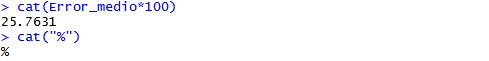
\includegraphics[width=0.7\linewidth]{error8a}
	\caption{Error ejercicio 8 (1)}
	\label{fig:error8a}
	\end{figure}
	
	El error es así de alto debido a que, además de que la función es no lineal, estamos también aplicando ruido a las etiquetas, por lo que se dificulta más aún el proceso de aprendizaje.
	\\
	\\
	A continuación procedemos a linealizar el problema. Para ello tomamos como vector de características (1,x1,x2,x1x2,x1^2, x2^2).
	
	\begin{lstlisting}
	muestra_8 <- simula_unif(N=1000, dim=2, c(-10,10))
	muestra_8 <- t(muestra_8)
	muestra_8 <- as.data.frame(muestra_8)
	names(muestra_8) <- c("x1","x2")
	#creo la nueva muestra con las variables del enunciado
	muestra_8_b <- data.frame(muestra_8$x2^2, muestra_8$x1^2, muestra_8$x1*muestra_8$x2, muestra_8$x2, muestra_8$x1, rep(1, nrow(muestra_8)))
	label_8_b <- (muestra_8$x1^2)+(muestra_8$x2^2)-25.0
	label_8_b[label_8_b>0] <- 1
	label_8_b[label_8_b<0] <- -1
	probs <- rep(1,length(label_8_b))
	ind_aleatorios <- sample(x=(1:length(label_8_b)), prob=probs, size=length(label_8_b)/10)
	#Le cambio el signo a la muestra aleatoria elegida
	label_8_b[ind_aleatorios] <- label_8_b[ind_aleatorios]*(-1)
	label_8_b <- matrix(label_8_b, ncol=1)
	#Ajusto la regresión lineal
	pesos <- Regress_lin(datos=muestra_8_b, label=label_8_b)
	label_test_8b <- evaluacion(x=muestra_8_b, w=pesos)
	errores <- label_test_8b!=as.vector(label_8_b)
	errores <- label_test_8b[errores]
	Error <- length(errores)/1000
	
	cat("Los pesos obtenidos son: ")
	cat(pesos)
	cat("\n")
	\end{lstlisting}
	
	En este código realizo lo mismo que anteriormente; genero una muestra aleatoria, la etiqueto con la función dada en el enunciado aplicándole ruido, y posteriormente creo otro conjunto de datos con el vector de características que nos dice el apartado. Con este conjunto de datos y las etiquetas calculadas realizamos la regresión lineal. En este apartado no he calculado el error ya que no nos lo pide.
	\\
	\\
	En el siguiente apartado ya sí tenemos que calcular el error fuera de la muestra. Realizamos el mismo procedimiento y posteriormente creamos una nueva muestra y le aplicamos la función f para crear la etiqueta y después la etiquetamos con los pesos tras la regresión lineal (en esta muestra no genero ruido). Después obtenemos un error sobre el 7\%.
	\begin{lstlisting}
	Error <- vector()
	for(i in 1:1000)
	{
		#Genero una muestra aleatoria a partir de la cual aprenderé
		muestra_8 <- simula_unif(N=1000, dim=2, c(-10,10))
		muestra_8 <- t(muestra_8)
		muestra_8 <- as.data.frame(muestra_8)
		names(muestra_8) <- c("x1","x2")
		#creo la nueva muestra con las variables del enunciado
		muestra_8_c <- data.frame(muestra_8$x2^2, muestra_8$x1^2, muestra_8$x1*muestra_8$x2, muestra_8$x1, muestra_8$x2, rep(1, nrow(muestra_8)))
		label_8_c <- muestra_8$x1^2+muestra_8$x2^2-25.0
		label_8_c[label_8_c>0] <- 1
		label_8_c[label_8_c<0] <- -1
		probs <- rep(1,length(label_8_c))
		ind_aleatorios <- sample(x=(1:length(label_8_c)), prob=probs, size=length(label_8_c)/10)
		#Le cambio el signo a la muestra aleatoria elegida
		label_8_c[ind_aleatorios] <- label_8_c[ind_aleatorios]*(-1)
		label_8_c <- matrix(label_8_c, ncol=1)
		pesos_8c <- Regress_lin(datos=muestra_8_c, label=label_8_c)
		#Genero la muestra con la que averiguaré el error fuera de la muestra
		muestra_8_out <- simula_unif(N=1000, dim=2, c(-10,10))
		muestra_8_out <- t(muestra_8_out)
		muestra_8_out <- as.data.frame(muestra_8_out)
		names(muestra_8_out) <- c("x1","x2")
		#Calculo su etiquetado para la función f
		label_8_out <- muestra_8_out$x1^2+muestra_8_out$x2^2-25.0
		label_8_out[label_8_out>0] <- 1
		label_8_out[label_8_out<0] <- -1
		#Convierto el conjunto de variables para linealizar la función
		muestra_8_out <- data.frame(muestra_8_out$x2^2, muestra_8_out$x1^2, muestra_8_out$x1*muestra_8_out$x2, muestra_8_out$x1, muestra_8_out$x2, rep(1, nrow(muestra_8_out)))
		#Evalúo con los pesos obtenidos anteriormente
		label_test_8 <- evaluacion(x=muestra_8_out, w=pesos_8c)
		errores <- label_8_out!=label_test_8
		errores <- label_8_out[errores]
		Error[i] <- length(errores)/1000
	}
	\end{lstlisting}
	Como vemos obtenemos mucho menos error que en el primer apartado. Esto es debido a que hemos linealizado el problema. Además, si no hubiese ruido en las etiquetas con las que aprendemos, el error sería bastante más bajo.
	\begin{figure} [H]
	\centering
	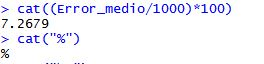
\includegraphics[width=0.7\linewidth]{error8c}
	\caption{Error ejercicio 8(2)}
	\label{fig:error8c}
	\end{figure}
	
	\section{Conclusiones}
	Como hemos visto PLA es un buen algoritmo de aprendizaje para datos linealmente separables. Si los datos no presentan una separabilidad lineal o ruido, el proceso de aprendizaje resulta de menos calidad, aunque podemos 'optimizar' el error usando variaciones como Pocket PLA. 
	\\
	\\
	En cuanto a la regresión lineal, también obtenemos buenas soluciones, ya que lo que hace es optimizar el error de dentro de la muestra. Además, combinado con PLA puede dar muy buenos resultados y resultar más eficiente al necesitar menos iteraciones el PLA para converger.

\end{document}